This section contains information needed to understand the project and the related work.

%\subsection{Kronecker graph}
%The graph that is used by the Graph500 is the Kronecker graph\cite{leskovec2010kronecker}. This is because a Kronecker graph has some nice properties which are also seen in graph that can be seen in the real world.
%TODO list of properties which are important to the graph500.
%TODO Say something about the properties of the graph. is a tree, so undirected.



\subsection{Graph 500 Benchmark 1 ("Search")}
Benchmark 1 ("Search")\cite{graph500-specs} consists of two kernels accessing a single data structure representing an undirected graph. These kernels are: the construction of the graph from an edge list and a search through the constructed graph. 

The benchmark has defined a few different problem classes. These are shown in table \ref{tab:problem_scales}. 
\begin{table}[!h]
	\begin{center}
	\begin{tabular}{|l|l|l|l|}
		\hline
		Problem class     & Scale & Edgefactor & Approx. Storage size in TB \\ \hline
		Toy (level 10)    & 26    & 16          & 0.0172                     \\ \hline
		Mini (level 11)   & 29    & 16          & 0.1374                     \\ \hline
		Small (level 12)  & 32    & 16          & 1.0995                     \\ \hline
		Medium (level 13) & 36    & 16          & 17.5922                    \\ \hline
		Large (level 14)  & 39    & 16          & 140.7375                   \\ \hline
		Huge (level 15)   & 42    & 16          & 1125.8999                  \\ \hline
	\end{tabular}
	\caption{The lists of problem classes as defined by the Graph 500, assuming the storage of the edge list is done n a 64-bit integer.}
	\label{tab:problem_scales}
	\end{center}
\end{table}
These problem classes give a sense of the size of the graph and the amount of storage needed to run the benchmark. The scale is defined as a combination of the amount of vertices and the edges connected to each of these vertices. The number of vertices is given by the scale. For example, the Toy problem is a graph of  $2^26$ vertices. The other parameter is the edgefactor. The edgefactor is ratio of edges to vertices. For each of the problem classes the edgefactor has been set to 16. 

The benchmark consists of the following steps:
\begin{enumerate}
	\item Generate the edge list.
	\item Construct a graph from the edge list.
	\item Randomly sample 64 unique search keys.
	\item For each search key:
	\begin{enumerate}
		\item Do the Breadth First Search and store all all visited vertices in an array.
		\item Validate that the array is a correct BFS search tree for the given search tree.
	\end{enumerate}
	\item Compute the performance
\end{enumerate}

In the following subsections all steps of the benchmark are explained in more detail.

\subsubsection{Generating the edge list}
The first step of the benchmark is generating the edge list. For this a data generator is used. The data generator constructs a list of edge tuples containing the start and end vertex, but also contains a vertex identifiers, thereby creating a list of undirected edges.

The intent of the graph generation is to convert a the edge list, which has no locality, into a data structure which can more easily be used. The list of generated tuples could have some locality because of the way the edges are generated. To lose this locality the edge list is randomized before inserted into the graph generation kernel. 

The data generator is a Kronecker generator, which has many properties which are seen in graphs in the real world\cite{leskovec2010kronecker}.

\subsubsection{Graph Construction}
The graph construction is the first timed kernel. The kernel takes the previously created edge list and transforms it into a data structure of choice. Examples of data structures to store graphs are Compressed Row Storage(CRS) and Compressed Sparse Column(CSC)\cite{ccs,crs}. The kernel takes only two parameters, the edge list and the size of the edge list. The number of vertices and other information that might be inferred from the edge list must computed by the kernel. 

One thing to note is that the data structure created in this kernel cannot be altered by subsequent kernels. 

\subsubsection{Sampling 64 search keys}
After the graph is constructed a 64 searches need to be done. By performing these searches the speed of traversal can be measured. The search keys need to have at least one other vertex connected to them, to prevent trivial searches. The search is done in a Breadth First Search way.

\subsubsection{Breadth First Search}
Breadth First Search\cite{bfs} (BFS) is the graph traversal which has been chosen by the Graph 500. BFS visits all vertices each on the level before moving on to the next level. It keeps traversing the Graph 500 until all levels in the graph have been visited. The level of a vertex is defined as the minimum number of edges that need to traversed to get to the root. An example of the traversal can be seen in figure \ref{fig:bfs}. 
Note that the Graph 500 benchmark only specifies the end results is a BFS, but does not specify how the program gets to this result.
\begin{figure}[!h]
	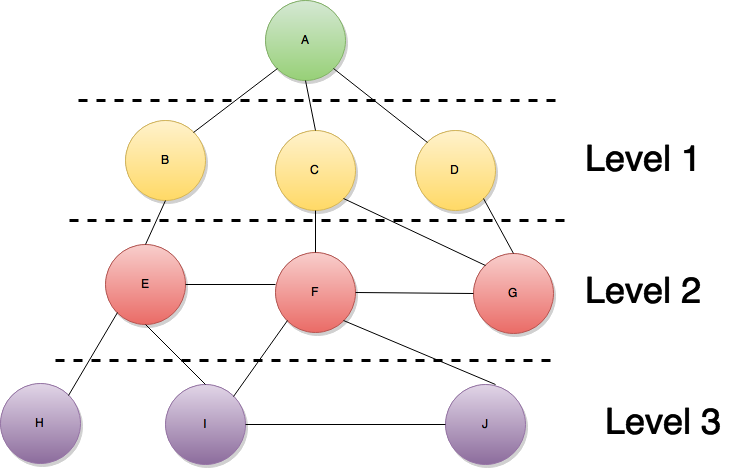
\includegraphics[width=\textwidth]{images/BFS-example1-with-levels}
	\caption{An example of BFS traversal is shown here. The nodes are traversed in alphabetical order.}
	\label{fig:bfs}
\end{figure}

\subsubsection{Validation}
After the each of the 64 searches a validation is done. The validation does soft checking of the results. Because there randomness in the process, validation against a reference is not possible. The validation checks for the following things:
\begin{enumerate}
\item The BFS tree is a tree and does not contain cycles.
\item Each tree edge connects vertices whose BFS levels differ by exactly one.
\item Every edge in the input list has vertices with levels that differ by at most one or that both are not in the BFS tree.
\item The BFS tree spans an entire connected component's vertices.
\item A node and its parent are joined by an edge of the original graph.
\end{enumerate}


\subsubsection{Timing and Performance metrics}
In code snippet \ref{lst:output} the output of the \texttt{graph500\_mpi\_simple}.
\begin{lstlisting}[label={lst:output}, caption= {Output of the benchmark.}]
SCALE:                          24
edgefactor:                     16
NBFS:                           64
graph_generation:               16.2365
num_mpi_processes:              8
construction_time:              15.4957
min_time:                       13.9349
firstquartile_time:             15.6177
median_time:                    15.7516
thirdquartile_time:             15.8136
max_time:                       16.1873
mean_time:                      15.6812
stddev_time:                    0.318657
min_nedge:                      268435456
firstquartile_nedge:            268435456
median_nedge:                   268435456
thirdquartile_nedge:            268435456
max_nedge:                      268435456
mean_nedge:                     268435456
stddev_nedge:                   0
min_TEPS:                       1.65831e+07
firstquartile_TEPS:             1.6975e+07
median_TEPS:                    1.70418e+07
thirdquartile_TEPS:             1.71879e+07
max_TEPS:                       1.92635e+07
harmonic_mean_TEPS:             1.71183e+07
harmonic_stddev_TEPS:           43826.4
\end{lstlisting}

The most important values from this output are:
\begin{description}
\item[SCALE] Is the size of the graph used in the benchmark.
\item[edgefactor] The edgefactor used in the graph.
\item[NBFS] Number of BFS searches run.
\item[graph\_generation] Time for the edge list generation.
\item[construction\_time] Time for first kernel.
\item[num\_mpi\_processes] The number of processes used for this benchmark. It does not specify how many nodes were used.
\item[harmonic mean TEPS] Mean  of the kernel 2 TEPS. Note: Because TEPS is a rate, the rates are compared using harmonic means\cite{harmonic_mean}.
\end{description}

The timing of the BFS starts right before visiting the root and ends when search has written the last value to the memory. The metric used to define the performance is called traversed edges per second (TEPS). The TEPS are measured through the benchmarking of kernel 2. The equations is.
\begin{equation}
TEPS(n) = total\_number\_ of\_edges / time\_of\_kernel\_2
\end{equation}
%\\


%\subsection{Graph compression}
%\label{back:compression}
%Sparse matrices are easy to compress because they consist of mostly zeros. 




%For example, if s $=$ 32 and n $=$ 128 (128 MPI processes), then the total communication 
%data volume $C(128, M)$ is calculated as $2^{32}$ $*$ 16 $*$ 2 $*$ $(127/128)$ $*$ 2 $*$ 8 = 2032 GB (2 TB). As previously noted, the entire graph for M(32) was 
%1.03 TB, so the amount of data was doubled.


